\documentclass[DIV=14,titlepage=false]{scrreprt}
%%%%%%%%%%%%%%%%%%%%%%%%%%%%%%%%%%%%%%%%%%%%%%%%%%%%%%%%%%%%%%%%%%%%%%%%%%%%%%%
%                                Basic Packages                               %
%%%%%%%%%%%%%%%%%%%%%%%%%%%%%%%%%%%%%%%%%%%%%%%%%%%%%%%%%%%%%%%%%%%%%%%%%%%%%%%
% Gives us multiple colors.
\usepackage[usenames,dvipsnames,pdftex]{xcolor}
% Lets us style link colors.
\usepackage{hyperref}
% Lets us import images and graphics.
\usepackage{graphicx}
% Lets us use figures in floating environments.
\usepackage{float}
% Lets us create multiple columns.
\usepackage{multicol}
% Gives us better math syntax.
\usepackage{amsmath,amsfonts,mathtools,amsthm,amssymb}
% Lets us strikethrough text.
\usepackage{cancel}
% Lets us edit the caption of a figure.
\usepackage{caption}
% Lets us import pdf directly in our tex code.
\usepackage{pdfpages}
% Lets us do algorithm stuff.
\usepackage[ruled,vlined,linesnumbered]{algorithm2e}
% Gets rid of some errors.
\usepackage{scrhack}
\def\class{article}
\usepackage{geometry}
\geometry{margin=0.9in}
%%%%%%%%%%%%%%%%%%%%%%%%%%%%%%%%%%%%%%%%%%%%%%%%%%%%%%%%%%%%%%%%%%%%%%%%%%%%%%%
%                                Basic Settings                               %
%%%%%%%%%%%%%%%%%%%%%%%%%%%%%%%%%%%%%%%%%%%%%%%%%%%%%%%%%%%%%%%%%%%%%%%%%%%%%%%

%%%%%%%%%%%%%
%  Symbols  %
%%%%%%%%%%%%%

\let\implies\Rightarrow
\let\impliedby\Leftarrow
\let\iff\Leftrightarrow
\let\epsilon\varepsilon

%%%%%%%%%%%%
%  Tables  %
%%%%%%%%%%%%

\setlength{\tabcolsep}{5pt}
\renewcommand\arraystretch{1.5}

%%%%%%%%%%%%%%%%%%%%%%%
%  Center Title Page  %
%%%%%%%%%%%%%%%%%%%%%%%

\usepackage{titling}
\renewcommand\maketitlehooka{\null\mbox{}\vfill}
\renewcommand\maketitlehookd{\vfill\null}

%%%%%%%%%%%%%%%%%%%%%%%%%%%%%%%%%%%%%%%%%%%%%%%%%%%%%%%
%  Create a grey background in the middle of the PDF  %
%%%%%%%%%%%%%%%%%%%%%%%%%%%%%%%%%%%%%%%%%%%%%%%%%%%%%%%

\usepackage{eso-pic}
\newcommand\definegraybackground{
  \definecolor{reallylightgray}{HTML}{FAFAFA}
  \AddToShipoutPicture{
    \ifthenelse{\isodd{\thepage}}{
      \AtPageLowerLeft{
        \put(\LenToUnit{\dimexpr\paperwidth-222pt},0){
          \color{reallylightgray}\rule{222pt}{297mm}
        }
      }
    }
    {
      \AtPageLowerLeft{
        \color{reallylightgray}\rule{222pt}{297mm}
      }
    }
  }
}

%%%%%%%%%%%%%%%%%%%%%%%%
%  Modify Links Color  %
%%%%%%%%%%%%%%%%%%%%%%%%

\hypersetup{
  % Enable highlighting links.
  colorlinks,
  % Change the color of links to blue.
  linkcolor={black},
  % Change the color of citations to black.
  citecolor={black},
  % Change the color of url's to blue with some black.
  urlcolor=blue
}

%%%%%%%%%%%%%%%%%%
% Fix WrapFigure %
%%%%%%%%%%%%%%%%%%

\newcommand{\wrapfill}{\par\ifnum\value{WF@wrappedlines}>0
    \parskip=0pt
    \addtocounter{WF@wrappedlines}{-1}%
    \null\vspace{\arabic{WF@wrappedlines}\baselineskip}%
    \WFclear
\fi}

%%%%%%%%%%%%%%%%%
% Multi Columns %
%%%%%%%%%%%%%%%%%

\let\multicolmulticols\multicols
\let\endmulticolmulticols\endmulticols

\RenewDocumentEnvironment{multicols}{mO{}}
{%
  \ifnum#1=1
    #2%
  \else % More than 1 column
    \multicolmulticols{#1}[#2]
  \fi
}
{%
  \ifnum#1=1
\else % More than 1 column
  \endmulticolmulticols
\fi
}

\newlength{\thickarrayrulewidth}
\setlength{\thickarrayrulewidth}{5\arrayrulewidth}

%%%%%%%%%%%%%%%%%%%%
%  Import Figures  %
%%%%%%%%%%%%%%%%%%%%

\usepackage{import}
\pdfminorversion=7

% EXAMPLE:
% 1. \incfig{limit-graph}
% 2. \incfig[0.4]{limit-graph}
% Parameters:
% 1. The figure name. It should be located in figures/NAME.tex_pdf.
% 2. (Optional) The width of the figure. Example: 0.5, 0.35.
\newcommand\incfig[2][1]{%
  \def\svgwidth{#1\columnwidth}
  \import{./figures/}{#2.pdf_tex}
}

\begingroup\expandafter\expandafter\expandafter\endgroup
\expandafter\ifx\csname pdfsuppresswarningpagegroup\endcsname\relax
\else
  \pdfsuppresswarningpagegroup=1\relax
\fi

%%%%%%%%%%%%%
%  Correct  %
%%%%%%%%%%%%%

% EXAMPLE:
% 1. \correct{INCORRECT}{CORRECT}
% Parameters:
% 1. The incorrect statement.
% 2. The correct statement.
\definecolor{correct}{HTML}{009900}
\newcommand\correct[2]{{\color{red}{#1 }}\ensuremath{\to}{\color{correct}{ #2}}}



\newcommand{\R}{\mathbb{R}}
\newcommand{\Z}{\mathbb{Z}}
\newcommand{\E}{\mathbb{E}}
\newcommand{\B}{\ensuremath{\mathcal{B}}}
\newcommand{\X}{\ensuremath{\mathcal{X}}}
\newcommand{\Y}{\ensuremath{\mathcal{Y}}}
\newcommand{\mA}{\ensuremath{\mathbf{A}}}
\newcommand{\mB}{\ensuremath{\mathbf{B}}}
\newcommand{\mC}{\ensuremath{\mathbf{C}}}
\newcommand{\mD}{\ensuremath{\mathbf{D}}}
\newcommand{\mX}{\ensuremath{\mathbf{X}}}
\newcommand{\mY}{\ensuremath{\mathbf{Y}}}
\newcommand{\mx}{\ensuremath{\mathbf{x}}}
\newcommand{\my}{\ensuremath{\mathbf{y}}}
\newcommand{\mI}{\ensuremath{\mathbf{I}}}
\newcommand{\mi}{\ensuremath{\mathbf{\iota}}}
\newcommand{\mmu}{\ensuremath{\mathbf{\mu}}}
\newcommand{\mc}{\ensuremath{\mathbf{c}}}
\newcommand{\mSigma}{\ensuremath{\mathbf{\Sigma}}}
\newcommand{\mzero}{\ensuremath{\mathbf{0}}}
\newcommand{\independent}{\perp\!\!\!\!\perp} 
\setlength{\parindent}{0pt}
%%%%%%%%%%%%%%%%%%%%%%%%%%%%%%%%%%%%%%%%%%%%%%%%%%%%%%%%%%%%%%%%%%%%%%%%%%%%%%%
%                                 Environments                                %
%%%%%%%%%%%%%%%%%%%%%%%%%%%%%%%%%%%%%%%%%%%%%%%%%%%%%%%%%%%%%%%%%%%%%%%%%%%%%%%

\usepackage{varwidth}
\usepackage{thmtools}
\usepackage[most,many,breakable]{tcolorbox}

\tcbuselibrary{theorems,skins,hooks}
\usetikzlibrary{arrows,calc,shadows.blur}

%%%%%%%%%%%%%%%%%%%
%  Define Colors  %
%%%%%%%%%%%%%%%%%%%

\definecolor{myblue}{RGB}{45, 111, 177}
\definecolor{mygreen}{RGB}{56, 140, 70}
\definecolor{myred}{RGB}{199, 68, 64}
\definecolor{mypurple}{RGB}{197, 92, 212}

\definecolor{definition}{HTML}{228b22}
\definecolor{theorem}{HTML}{00007B}
\definecolor{example}{HTML}{2A7F7F}
\definecolor{definition}{HTML}{228b22}
\definecolor{prop}{HTML}{191971}
\definecolor{lemma}{HTML}{983b0f}
\definecolor{exercise}{HTML}{88D6D1}

\colorlet{definition}{mygreen!85!black}
\colorlet{claim}{mygreen!85!black}
\colorlet{corollary}{mypurple!85!black}
\colorlet{proof}{theorem}

%%%%%%%%%%%%%%%%%%%%%%
%  Helpful Commands  %
%%%%%%%%%%%%%%%%%%%%%%

% EXAMPLE:
% 1. \createnewtheoremstyle{thmdefinitionbox}{}{}
% 2. \createnewtheoremstyle{thmtheorembox}{}{}
% 3. \createnewtheoremstyle{thmproofbox}{qed=\qedsymbol}{
%       rightline=false, topline=false, bottomline=false
%    }
% Parameters:
% 1. Theorem name.
% 2. Any extra parameters to pass directly to declaretheoremstyle.
% 3. Any extra parameters to pass directly to mdframed.
\newcommand\createnewtheoremstyle[3]{
  \declaretheoremstyle[
  headfont=\bfseries\sffamily, bodyfont=\normalfont, #2,
  mdframed={
    #3,
  },
  ]{#1}
}

% EXAMPLE:
% 1. \createnewcoloredtheoremstyle{thmdefinitionbox}{definition}{}{}
% 2. \createnewcoloredtheoremstyle{thmexamplebox}{example}{}{
%       rightline=true, leftline=true, topline=true, bottomline=true
%     }
% 3. \createnewcoloredtheoremstyle{thmproofbox}{proof}{qed=\qedsymbol}{backgroundcolor=white}
% Parameters:
% 1. Theorem name.
% 2. Color of theorem.
% 3. Any extra parameters to pass directly to declaretheoremstyle.
% 4. Any extra parameters to pass directly to mdframed.
\newcommand\createnewcoloredtheoremstyle[4]{
  \declaretheoremstyle[
  headfont=\bfseries\sffamily\color{#2}, bodyfont=\normalfont, #3,
  mdframed={
    linewidth=2pt,
    rightline=false, leftline=true, topline=false, bottomline=false,
    linecolor=#2, backgroundcolor=#2!5, #4,
  },
  ]{#1}
}

%%%%%%%%%%%%%%%%%%%%%%%%%%%%%%%%%%%
%  Create the Environment Styles  %
%%%%%%%%%%%%%%%%%%%%%%%%%%%%%%%%%%%

\makeatletter
\@ifclasswith\class{nocolor}{
  % Environments without color.

  \createnewtheoremstyle{thmdefinitionbox}{}{}
  \createnewtheoremstyle{thmtheorembox}{}{}
  \createnewtheoremstyle{thmexamplebox}{}{}
  \createnewtheoremstyle{thmclaimbox}{}{}
  \createnewtheoremstyle{thmcorollarybox}{}{}
  \createnewtheoremstyle{thmpropbox}{}{}
  \createnewtheoremstyle{thmlemmabox}{}{}
  \createnewtheoremstyle{thmexercisebox}{}{}
  \createnewtheoremstyle{thmdefinitionbox}{}{}
  \createnewtheoremstyle{thmquestionbox}{}{}
  \createnewtheoremstyle{thmsolutionbox}{}{}

  \createnewtheoremstyle{thmproofbox}{qed=\qedsymbol}{}
  \createnewtheoremstyle{thmexplanationbox}{}{}
}{
  % Environments with color.

  \createnewcoloredtheoremstyle{thmdefinitionbox}{definition}{}{}
  \createnewcoloredtheoremstyle{thmtheorembox}{theorem}{}{}
  \createnewcoloredtheoremstyle{thmexamplebox}{example}{}{
    rightline=true, leftline=true, topline=true, bottomline=true
  }
  \createnewcoloredtheoremstyle{thmclaimbox}{claim}{}{}
  \createnewcoloredtheoremstyle{thmcorollarybox}{corollary}{}{}
  \createnewcoloredtheoremstyle{thmpropbox}{prop}{}{}
  \createnewcoloredtheoremstyle{thmlemmabox}{lemma}{}{}
  \createnewcoloredtheoremstyle{thmexercisebox}{exercise}{}{}

  \createnewcoloredtheoremstyle{thmproofbox}{proof}{qed=\qedsymbol}{backgroundcolor=white}
  \createnewcoloredtheoremstyle{thmexplanationbox}{example}{qed=\qedsymbol}{backgroundcolor=white}
}
\makeatother

%%%%%%%%%%%%%%%%%%%%%%%%%%%%%
%  Create the Environments  %
%%%%%%%%%%%%%%%%%%%%%%%%%%%%%

\declaretheorem[numberwithin=section, style=thmtheorembox,     name=Theorem]{theorem}
\declaretheorem[numbered=no,          style=thmexamplebox,     name=Example]{example}
\declaretheorem[numberwithin=section, style=thmclaimbox,       name=Claim]{claim}
\declaretheorem[numberwithin=section, style=thmcorollarybox,   name=Corollary]{corollary}
\declaretheorem[numberwithin=section, style=thmpropbox,        name=Proposition]{prop}
\declaretheorem[numberwithin=section, style=thmlemmabox,       name=Lemma]{lemma}
\declaretheorem[numberwithin=section, style=thmexercisebox,    name=Exercise]{exercise}
\declaretheorem[numbered=no,          style=thmproofbox,       name=Proof]{replacementproof}
\declaretheorem[numbered=no,          style=thmexplanationbox, name=Proof]{expl}

\makeatletter
\@ifclasswith\class{nocolor}{
  % Environments without color.

  \newtheorem*{note}{Note}

  \declaretheorem[numberwithin=section, style=thmdefinitionbox, name=Definition]{definition}
  \declaretheorem[numberwithin=section, style=thmquestionbox,   name=Question]{question}
  \declaretheorem[numberwithin=section, style=thmsolutionbox,   name=Solution]{solution}
}{
  % Environments with color.

  \newtcbtheorem[number within=section]{Definition}{Definition}{
    enhanced,
    before skip=2mm,
    after skip=2mm,
    colback=red!5,
    colframe=red!80!black,
    colbacktitle=red!75!black,
    boxrule=0.5mm,
    attach boxed title to top left={
      xshift=1cm,
      yshift*=1mm-\tcboxedtitleheight
    },
    varwidth boxed title*=-3cm,
    boxed title style={
      interior engine=empty,
      frame code={
        \path[fill=tcbcolback]
        ([yshift=-1mm,xshift=-1mm]frame.north west)
        arc[start angle=0,end angle=180,radius=1mm]
        ([yshift=-1mm,xshift=1mm]frame.north east)
        arc[start angle=180,end angle=0,radius=1mm];
        \path[left color=tcbcolback!60!black,right color=tcbcolback!60!black,
        middle color=tcbcolback!80!black]
        ([xshift=-2mm]frame.north west) -- ([xshift=2mm]frame.north east)
        [rounded corners=1mm]-- ([xshift=1mm,yshift=-1mm]frame.north east)
        -- (frame.south east) -- (frame.south west)
        -- ([xshift=-1mm,yshift=-1mm]frame.north west)
        [sharp corners]-- cycle;
      },
    },
    fonttitle=\bfseries,
    title={#2},
    #1
  }{def}

  \NewDocumentEnvironment{definition}{O{}O{}}
    {\begin{Definition}{#1}{#2}}{\end{Definition}}

  \newtcolorbox{note}[1][]{%
    enhanced jigsaw,
    colback=gray!20!white,%
    colframe=gray!80!black,
    size=small,
    boxrule=1pt,
    title=\textbf{Note:-},
    halign title=flush center,
    coltitle=black,
    breakable,
    drop shadow=black!50!white,
    attach boxed title to top left={xshift=1cm,yshift=-\tcboxedtitleheight/2,yshifttext=-\tcboxedtitleheight/2},
    minipage boxed title=1.5cm,
    boxed title style={%
      colback=white,
      size=fbox,
      boxrule=1pt,
      boxsep=2pt,
      underlay={%
        \coordinate (dotA) at ($(interior.west) + (-0.5pt,0)$);
        \coordinate (dotB) at ($(interior.east) + (0.5pt,0)$);
        \begin{scope}
          \clip (interior.north west) rectangle ([xshift=3ex]interior.east);
          \filldraw [white, blur shadow={shadow opacity=60, shadow yshift=-.75ex}, rounded corners=2pt] (interior.north west) rectangle (interior.south east);
        \end{scope}
        \begin{scope}[gray!80!black]
          \fill (dotA) circle (2pt);
          \fill (dotB) circle (2pt);
        \end{scope}
      },
    },
    #1,
  }

  \newtcbtheorem{Question}{Question}{enhanced,
    breakable,
    colback=white,
    colframe=myblue!80!black,
    attach boxed title to top left={yshift*=-\tcboxedtitleheight},
    fonttitle=\bfseries,
    title=\textbf{Question:-},
    boxed title size=title,
    boxed title style={%
      sharp corners,
      rounded corners=northwest,
      colback=tcbcolframe,
      boxrule=0pt,
    },
    underlay boxed title={%
      \path[fill=tcbcolframe] (title.south west)--(title.south east)
      to[out=0, in=180] ([xshift=5mm]title.east)--
      (title.center-|frame.east)
      [rounded corners=\kvtcb@arc] |-
      (frame.north) -| cycle;
    },
    #1
  }{def}

  \NewDocumentEnvironment{question}{O{}O{}}
  {\begin{Question}{#1}{#2}}{\end{Question}}

  \newtcolorbox{Solution}{enhanced,
    breakable,
    colback=white,
    colframe=mygreen!80!black,
    attach boxed title to top left={yshift*=-\tcboxedtitleheight},
    title=\textbf{Solution:-},
    boxed title size=title,
    boxed title style={%
      sharp corners,
      rounded corners=northwest,
      colback=tcbcolframe,
      boxrule=0pt,
    },
    underlay boxed title={%
      \path[fill=tcbcolframe] (title.south west)--(title.south east)
      to[out=0, in=180] ([xshift=5mm]title.east)--
      (title.center-|frame.east)
      [rounded corners=\kvtcb@arc] |-
      (frame.north) -| cycle;
    },
  }

  \NewDocumentEnvironment{solution}{O{}O{}}
  {\vspace{-10pt}\begin{Solution}{#1}{#2}}{\end{Solution}}
}
\makeatother

%%%%%%%%%%%%%%%%%%%%%%%%%%%%
%  Edit Proof Environment  %
%%%%%%%%%%%%%%%%%%%%%%%%%%%%

\renewenvironment{proof}[1][\proofname]{\vspace{-10pt}\begin{replacementproof}}{\end{replacementproof}}
\newenvironment{explanation}[1][\proofname]{\vspace{-10pt}\begin{expl}}{\end{expl}}

\theoremstyle{definition}

\newtheorem*{notation}{Notation}
\newtheorem*{previouslyseen}{As previously seen}
\newtheorem*{problem}{Problem}
\newtheorem*{observe}{Observe}
\newtheorem*{property}{Property}
\newtheorem*{intuition}{Intuition}

\setuptoc{toc}{leveldown}

\begin{document}
\pagenumbering{gobble}
\vspace{-10pt}
\setcounter{chapter}{6}


\chapter{Nonlinear Models}
Non-linearities can enter a model in a variety of ways. Some common examples are:
\begin{itemize}
    \item ARMA models with multiplicative terms:
     \[
        ,y_t = \phi y_{t-1} +\epsilon_t + \beta \epsilon_{t-1} y_{t-1}, \quad \epsilon_t \sim NID(0,\sigma^2)
    \]
    \item Nonlinear functional forms
    \item Non-Gaussian, EG disturbances follow a t-distribution
    \item Dynamics in scale rather than location (e.g. GARCH)
    \item Switching regimes
\end{itemize}
There are 2 broad classes of models, parameter-driven and observation-driven.\\
An observation driven model is set up in terms of conditional distribution for the $t$-th observation: $p(y_t|Y_{t-1}|\phi)$. THe likelihood function is immediately available.\\
A parameter driven model typically does not allow for a likelihood function, where we have some link function: $ y_t = \mu e^{\beta_t} + \epsilon_t, \quad \beta_t = \phi \beta_{t-1} + \eta_t$, here it is exponential.
\section{Nonlinear modelling and white noise}
\subsection{Law of iterated expectations}
\begin{definition}[Law of iterated expectations (LIE)]
    \[
        \E[y] = \E_x[\E[y|x]]
    \]
\end{definition}
\begin{proof}
    \[
        \E_x[\E[y|x]] = \int \left[ \int y p(y|x) dy \right] p(x) dx = \int \int y p(y,x) dy dx = \int y p(y) dy = \E[y]
    \]
\end{proof}
This is useful, since we can find a sequence of one step ahead expectations:
\[
    \E_{t-j}[g(y_t)] = \E_{t-j}\cdots \E_{t-1}[g(y_t)]
\]
where the unconditional expectation is found by letting $j \to \infty$.
\begin{exercise}
    Show
    \[
        Var[y] = \E_x[Var[y|x]] + Var_x[\E[y|x]]
    \]
\end{exercise}
\begin{solution}
\begin{align*}
    Var[y] &= \E[y^2] - \E[y]^2\\
    &= \E_x[\E[y^2|x]] - \E_x[\E[y|x]]^2\\
    &= \E_x[Var[y|x] + \E[y|x]^2] - \E_x[\E[y|x]]^2\\
    &= \E_x[Var[y|x]] + \E_x[\E[y|x]^2] - \E_x[\E[y|x]]^2\\
    &= \E_x[Var[y|x]] + Var[\E[y|x]]
\end{align*}
\end{solution}
\subsection{White noise}
\textbf{White noise} is uncorrelated, i.e. $\E[y_t y_s] = 0, \quad t \neq s$ with constant variance (and zero mean).\\
\textbf{Strict white noise} is stronger, we require independence, not just uncorrelatedness\footnote{These are the same with Gaussian noise, since the distribution is fully defined by the first 2 moments}.\\
\textbf{Martingale Difference} has a zero (or constant) conditional expectation:
\[
    \E_{t-1}[y_t] = 0
\]
and thus is uncorrelated with any function of past observations:
\[
    \E[y_t f(Y_{t-1})|Y_{t-1}] = f(Y_{t-1})\E[y_t|Y_{t-1}] = 0
\]
\begin{example}
    \[
        y_t = \epsilon_t + \beta \epsilon_{t-1} \epsilon_{t-2} \quad \epsilon_t \sim NID(0,\sigma^2)
    \]
    The autocovariance at lag $\tau$ can be derived as:
    \begin{align*}
        \E(y_t y_{t-\tau}) &= \E(\epsilon_t + \beta \epsilon_{t-1} \epsilon_{t-2} )(\epsilon_{t-\tau} + \beta \epsilon_{t-\tau-1} \epsilon_{t-\tau-2})\\
        &= \E(\epsilon_t \epsilon_{t-\tau}) + \beta \E(\epsilon_t \epsilon_{t-\tau-1} \epsilon_{t-\tau-2}) + \beta \E(\epsilon_{t-1} \epsilon_{t-\tau} \epsilon_{t-\tau-1}) + \beta^2 \E(\epsilon_{t-1} \epsilon_{t-2} \epsilon_{t-\tau} \epsilon_{t-\tau-1})\\
        &= 0 \quad \text{if} \quad \tau \neq 0
    \end{align*}
    Since all observations are uncorrelated the series is white noise, however the observations are not independent, the conditional mean is:
    \[
        \E_{t-1}[y_t] = \E_{t-1}[\epsilon_t] + \beta \E_{t-1}[\epsilon_{t-1} \epsilon_{t-2}] = \beta \epsilon_{t-1} \epsilon_{t-2}
    \]
    so the series is not a martingale difference.
\end{example}
\begin{example}[ARCH]
    \begin{align*}
        y_t &= \sigma_{t|t-1} \epsilon_t, \quad \epsilon_t \sim NID(0,1)\\
        \sigma_{t|t-1}^2 &= \gamma + \alpha y_{t-1}^2
    \end{align*}
    This is a Martingale difference since 
    \[
        \E_{t-1}[y_t] = \sigma_{t|t-1} \E_{t-1}[\epsilon_t] = 0
    \]
    implying it is also white noise.
\end{example}
\subsection{Linearity and Prediction}
When disturbances in an ARMA are IID, the MMSE predictor is the conditional mean. It is linear in the observations and disturbances.\\
Assuming instead that the disturbances are MDs with mean zero and constant variance, the MMSE predictor is again the conditional expectation by the LIE.\\
When disturbances are WN (not strict WN) the MMSE = MMSLE, however if disturbances are not independent the MMSE is not the MMSLE.
\begin{example}
    \[
        y_t = \epsilon_t + \beta \epsilon_{t-1} \epsilon_{t-2}, \quad \epsilon_t \sim NID(0,\sigma^2)
    \]
The MMSLE of future observations is zero, with MSE equal to the variance of future observations:
\begin{align*}
    Var(y_t) &= \E[\epsilon_t^2] + 2 \beta \E[\epsilon_t \epsilon_{t-1} \epsilon_{t-2}] + \beta^2 \E[\epsilon_{t-1}^2 \epsilon_{t-2}^2]\\
    &= \sigma^2 + 0 + \beta^2 \sigma^4 
\end{align*}
However the MMSE (the conditional mean) is:
\[
    \E[y_t|Y_{t-1}] = \beta \epsilon_{t-1} \epsilon_{t-2}
\]
which has MSE:
\[
    \E[y_t - \beta \epsilon_{t-1} \epsilon_{t-2}]^2 = \E[\epsilon_t]^2 = \sigma^2
\]
We can use the LIE to compute multi-step predictions:
\[
        \E_T[y_{T+\ell}] = \begin{cases*}
            \E_T[\beta \epsilon_{T} \epsilon_{T-1}] = \beta \epsilon_{T} \epsilon_{T-1} & $\ell = 1$\\
            \E_T[\beta \epsilon_{T+1} \epsilon_{T}] = 0 & $\ell = 2$\\
             0 & $\ell > 2$
        \end{cases*}
\]
\end{example}
\section{Stationarity}
\begin{theorem}[Krengel's Theorem]
If $y_t$ is strictly stationary and ergodic (SE) then a continuous transformation $g(y_t, y_{t-1}, \dots)$ is also SE. 
\end{theorem}
Weak stationarity of $g$ doesn't follow from weak stationarity of $y_t$ since the moments may not exist. E.g. if $y_t \sim t \nu$ then $g(y_t) = e^{y_t}$ has no finite moments.
\begin{definition}[Linear stochastic recurrence equation]
    \[
        y_{t+1} = x_t y_t + z_t 
    \]
    where $x_t$ and $z_t$ are strictly stationary and ergodic.
\end{definition}
\begin{theorem}
    The conditions:
    \begin{enumerate}
        \item $\E(\max(0, \ln |z_t|)) = \E(\ln ^+ |z_t|) < \infty$
        \item $\E(\ln|x_t|) < 0$
    \end{enumerate}
    are sufficient for the existence and uniqueness of a strictly stationary solution for $y_t$.
\end{theorem}
Condition 1 usually holds, it is the second condition that is important. It is known as the \textbf{contraction condition} and can be interpreted as saying that the $x_t$'s are on average smaller than 1 (in absolute value). We can see this by applying Jensen's inequality:
\[
    \E(\ln|x_t|) \leq \ln \E(|x_t|) \implies \E(|x_t|) < 1
\]
\begin{example}
    If $x_t$ is lognormal, $ln x_t \sim N(\mu, \sigma^2)$ the contraction condition is $\E(\ln x_t) = \mu < 0$, whereat $\E(x_t) = e^{\mu + \sigma^2/2}$, thus $\ln \E(x_t) = \mu + \sigma^2/2 > \mu$ is stronger than needed.
\end{example}
\begin{exercise}
    What is the stationarity condition for the bilinear model?
    \begin{equation}
        \label{eq:bilinear} y_t = \phi y_{t-1} + \epsilon_t + \beta \epsilon_{t-1} y_{t-1}
    \end{equation}
\end{exercise}
\begin{solution}
    We can write the model as:
    \[
        y_t= (\phi + \beta \epsilon_{t-1})y_{t-1} + \epsilon_t
    \]
    which is a SRE with $x_t = \phi + \beta \epsilon_{t-1}$ and $z_t = \epsilon_t$. The contraction condition is:
    \[
        \E(\ln|x_t|) = \E(\ln|\phi + \beta \epsilon_{t-1}|) < 0
    \]
\end{solution}
\subsection{Asymptotic Stationarity}
Consider a non-linear generalisation of the linear SRE above:
\[
    y_{t+1} = \mathbf{\varphi}(y_t, \mathbf{z}_t, \mathbf{\psi})
\]
where $\mathbf{z}_t$ is a vector of SE variables\footnote{When $\mathbf{z_t}$ is a vector of IID variables, the equation is known as a Markov system} and $\mathbf{\psi}$ is a vector of parameters.
\begin{theorem}[Bougerol's Theorem]
    If \begin{itemize}
        \item There exists $y_1$ such that $\E(\ln^+|\varphi(y_1, \mathbf{z}_1|)) < \infty$
        \item $\E(\ln \sup_y |\frac{\partial \varphi(y, \mathbf{z})}{\partial y}|) < 0$
    \end{itemize}
    then for any starting value $y_1$, a series $y_t$ converges exponentially and almost surely to a unique SE solution. In other words $|y_t(y_1,\mathbf{\psi}) - y_t(\mathbf{\psi})| \overset{e.a.s.}{\to} 0$ as $t \to \infty$.
\end{theorem}
Intuitively this just means that it doesn't matter where we start, we will always converge to the same solution. 
\begin{example}
    Consider this cursed AR(1) model:
    \[
        y_t = \phi \frac{e^{y_{t-1}}-1}{e^{y_{t-1}}+1} + \epsilon_t \quad \epsilon_t \sim NID(0,\sigma^2)
    \]
    Clearly
    \[
        -1 < \frac{e^{y_{t-1}}-1}{e^{y_{t-1}}+1} < 1
    \]
    so the first condition holds for any finite $y_1$. We now examine the second condition:
    \begin{align*}
        \left| \frac{\partial}{\partial y} \left(\phi \frac{e^y-1}{e^y+1} + \epsilon_t \right)\right| &= \left| \phi \frac{(e^y+1)e^y - (e^y-1)e^y}{(e^y+1)^2} \right|\\
        &= |\phi| \left| \frac{2e^y}{(e^y+1)^2} \right|\\
        &= |\phi| \frac{2e^y}{(e^y+1)^2}
    \end{align*}
    To solve for the supremum we take the derivative and set it to zero:
    \begin{align*}
        0 &= \frac{d}{dy} \frac{2e^y}{(e^y+1)^2} \\
        \implies 0 &= (e^y+1)^2e^y - 2e^y(e^y+1)e^y\\
        \implies e^y + 1 &= 2\\
        \implies y &= 0 \quad \text{with} \quad \frac{2e^y}{(e^y+1)^2} = \frac{1}{2}
    \end{align*}
    Thus:
    \[
        \E(\ln \sup_y |\frac{\partial \varphi(y, \mathbf{z})}{\partial y}|) = \E(\ln \frac{|\phi|}{2}) = \E(\ln |\phi|) - \ln 2 < 0 \equiv |\phi| < 2
    \]
\end{example}
\section{Distributions}
\begin{definition}[Survival function]
    \[
        S(y) = P(Y > y) = 1 - F(y)
    \]
\end{definition}
\begin{example}[Exponential]
    \[
        F(y) = 1 - e^{-y/\theta} \implies S(y) = e^{-y/\theta}
    \]
\end{example}
\begin{definition}[Probability integral transform]
The PIT of Y is the standard uniform, i.e. $F(Y) \sim U(0,1)$
\[
    f(F(Y)) = f(y) \frac{dy}{dF(y)} = 1
\]    
Thus we can generate any distribution by transforming a standard uniform.
\end{definition}
\begin{definition}[t-distribution]
    \[
        f(y) = \frac{\Gamma(\frac{\nu+1}{2})}{\sqrt{\nu \pi} \Gamma(\frac{\nu}{2})} \left(1 + \frac{(y-\mu)^2}{\nu \phi^2} \right)^{-\frac{\nu+1}{2}}
    \]    
    where $\mu$ is median and $\phi$ is scale.
\end{definition}
The location-dispersion model is:
\[
    y_t = \mu + \psi \epsilon_t
\]
where $\epsilon_t$ has mean zero, and $\psi$ is called the dispersion for $y_t$. For non-negative variables a location + scale model is needed:
\[
    y_t = \psi \epsilon_t
\]
where $\epsilon_t$ has mean one. When $y_t>0$ taking logarithms gives:
\[
    \ln y_t = \ln \psi + \ln \epsilon_t
\]
so $\ln \psi$ is now a location parameter.
\begin{definition}[Gamma distribution]
    A gamma($\psi, \gamma$) distribution has density:
    \[
        f(y) = \psi^{-\gamma} \frac{y^{\gamma-1}e^{-y/\psi}}{\Gamma(\gamma)}
    \]
    Where $\psi$ is the scale parameter and $\gamma$ is the shape parameter. The mean is $\gamma \psi$ and the variance is $\gamma \psi^2$.
\end{definition}
The chi-squared distribution is gamma($2, \nu/2$), setting $\gamma = 1$ gives an exponential distribution.
\begin{definition}[Log-logistic distribution]
    A log-logistic($\psi, \gamma$) distribution has density:
    \[
        f(y) = \frac{\nu \frac{y}{\psi}^{\nu-1}}{\psi \left(1 + \left(\frac{y}{\psi}\right)^\nu\right)^2}
    \]
\end{definition}
\begin{definition}[Quantiles]
    The $\alpha$-quantile of a distribution is the value $y_\alpha$ such that $F(y_\alpha) = \alpha$. The median is the 0.5-quantile.
\end{definition}
\begin{definition}[Heavy tails]
    A distribution is said to be heavy tailed if
    \[
        \underset{y \to \infty}{\lim} \exp(y/\alpha) S(y) = \infty \quad \forall \alpha > 0
    \]
\end{definition}
\begin{example}[Exponential distribution]
    $S(y) = e^{-y/\alpha}$ so 
    \[
        \exp(y/\alpha) S(y) = e^{y/\alpha} e^{-y/\alpha} = 1
    \]
    thus it is not heavy tailed.
\end{example}
\begin{definition}[Fat tails]
    A distribution is said to have fat tails if
    \[
        S(y) = c L(y)y^{-\alpha} \quad \alpha > 0
    \]
    where $L(y)$ is slowly varying, i.e. $\lim_{y \to \infty} L(\lambda y)/L(y) = 1$ for all $\lambda > 0$ and $c$ is a non-negative constant.
\end{definition}
\begin{claim}
    Fat tailed $\implies$ heavy tailed, but not the reverse.
\end{claim}
\section{Nonlinear state space models}
Parameter driven models may be nonlinear in the measurement equation, the transition equation or both. The basic model is:
\begin{align*}
    y_t &= f(\theta_t,\epsilon_t|\varphi)\\
    \theta_{t+1} &= \psi(\theta_t,\eta_t|\varphi)
\end{align*}
where $\theta$ is the signal, $\varphi$ parameters and $\epsilon,\eta$ disturbances with specified distributions.
\begin{example}[AR1 dynamic equation]
    Consider
    \begin{align*}
        y_t &= \mu \exp(\beta_t)+\epsilon_t \quad \epsilon_t \sim NID(0,\sigma^2_\epsilon) \\
        \beta_{t+1} &= \phi \beta_{t} + \eta_t \quad \eta_t \sim NID(0,\sigma^2_\eta) \quad |\phi|<1
    \end{align*}
    Clearly the state equation follows an AR1 with parameter less than 1, it is SE. We can thus apply Krengel's theorem to show that $y_t$ is also SE.
\end{example}
\begin{example}[Non-negativity]
    When $y_t$ is non-negative, any model must be non-linear. Consider the measurement equation below, with time varying mean $\mu_t$:
    \[
        y_t = \mu_t \epsilon_t \quad 0 \leq y_t < \infty  
    \]
    where $\epsilon_t$ has a gamma distribution with mean 1. We can use an exponential link function to model the logarithm of $mu_t$ to ensure $mu_t$ remains positive:
    \[
        \ln \mu_{t+1} = \delta + \phi \ln \mu_t + \alpha \eta_t
    \]
    The restriction $|phi|<1$ guarantees the stationarity of $\ln \mu_t$, and hence of $y_t$. 
\end{example}
We can also consider conditionally Gaussian state space models, allowing the possibility of feedback from past observations to the system matrices that would otherwise be a linear SSM. We can derive the Kalman filter exactly as before and construct the likelihood function since the system matrixes are fixed at time $t-1$. It is not usually possible to predict more than one-step ahead however.
\begin{example}
    An example of a conditionally Gaussian process is
    \[
        y_t = \phi_t y_{t-1} + \epsilon_t
    \]
    \[
        \phi_{t+1} = \phi (1-\alpha)+\alpha\phi_t+\eta_t
    \]
    where $\alpha$ is a fixed parameter. When $\phi_t$ is regarded as the state, we have a conditionally Gaussian SSM with $z=y_{t-1}$. When $|\alpha|<1$ the model is SE. 
\end{example}
\section{Observation driven models}
An observation driven model is set up to give a conditional distribution for each observation, that is:
\[
    p(y_t|Y_{t-1}|\varphi)
\]
where $Y_{t-1}$ denotes all past observations. We can then construct the likelihood in the usual way.
\begin{example}[Bilinear model]
    \[
        y_t = \phi y_{t-1} + \epsilon_t + \beta \epsilon_{t-1} y_{t-1}
    \]
    We can compute the ML estimate by minimising the SSR. Setting up the model in SSF:
    \begin{align*}
        y_t &= \mu_{t|t-1} + \epsilon_t\\
        \mu_{t+1|t} = \phi y_t + \beta \epsilon_t y_t = (\phi + \beta \epsilon_t)\mu_{t|t-1} + \phi \epsilon_t + \beta \epsilon_t^2
    \end{align*}
\end{example}
More general observation models can be written:
\[
    p(y_t | \alpha_{t|t-1}, Y_{t-1}|\varphi)
\]
with the transition equation becoming a filtering equation\[
    \alpha_{t+1|t} = g(\alpha_{t|t-1}, y_t, Y_{t-1}|\varphi)
\]
The signal $\theta$ is the dynamic parameter in the conditional distribution. It depends on $\alpha_{t+1|t}$ so \[
    \theta_{t|t-1} = h(\alpha_{t|t-1}, y_t, Y_{t-1}|\varphi)
    \]
    and we can write
    \[
        p(y_t|h(\alpha_{t|t-1}, Y_{t-1}|\varphi))   
    \]
Commonly it is useful to keep the state variable $\alpha$ positive, so we can use an exponential link function:
\[
    \alpha_{t+1|t} = e^{\theta_{t+1|t}}
\]
\subsection{Moment-driven and score-driven models}
In a moment-driven model the dynamic equation for the state is driven by observed $y_t$, E.G.:
\[
    \mu_{t+1|t} = \delta + \beta \mu_{t|t-1} + \alpha y_t
\]
The score-driven model is driven by the score of the conditional distribution, that is:
\[
    \mu_{t+1|t} = \lambda + \phi \mu_{t|t-1} + \kappa \left( k \frac{\partial \ln p(y_t|\mu_{t|t-1})}{\partial \mu_{t|t-1}} \right)
\]
Consider the linear Gaussian AR1N model. The finite sample Kalman filter begins at $t=1$ taking account of the uncertainty with a diffuse prior. However we might consider a model based on the steady-state (constant Kalman gain), but initialised at $t=1$. We write this as:
\[
    y_t = \mu + \mu_{t|t-1} + \nu_t
\]
\[
    \mu_{t+1|t} = \phi \mu_{t|t-1} + \kappa \nu_t
\]
where the innovations $\nu_t$  are NID and $\mu_{1|0}$ is fixed. We can write the filter as
\begin{align*}
    \mu_{t+1|t} &= \phi \mu_{t|t-1} + \kappa \nu_t\\
    &= \phi \mu_{t|t-1} + \kappa (y_t - \mu - \mu_{t|t-1})\\
    &= (\phi - \kappa)\mu_{t|t-1} + \kappa (y_t - \mu)
\end{align*}
Substituting repeatedly gives 
\[
    \mu{t+1|t} = \kappa \sum_{j=0}^{t-1} (\phi - \kappa)^j (y_{t-j} - \mu) + (\phi - \kappa)^t \mu_{1|0}
\]
Although the filter is typically started with $\mu_{1|0} = 0$, as long as $|\phi - \kappa | <1$ the filtered level will converge to the same value for any starting value.\\
In a score-driven model the dynamic equation for the above is driven by a variable that is proportional to the score of the conditional distribution, that is:
\[
    \mu_{t+1|t} = \phi \mu_{t|t-1} + \kappa \left( k \frac{\partial \ln p(y_t|\mu_{t|t-1})}{\partial \mu_{t|t-1}} \right)
    \]
The inverse of the information matrix is a common choice for $k$.
\begin{example}[Non-negativity - Gamma distribution]
    For non-negative variables we use a location-scale model. Suppose $p(y_t|\mu_{t|t-1}, \psi)$ is gamma with shape parameter $\gamma$ and evolving scale parameter $\mu_{t|t-1}$. 
    
    \textbf{Moment-driven Model}\\
    A filter for the scale can be written as:
    \[
        \mu_{t+1|t} = \delta + \beta \mu_{t|t-1} + \alpha y_t
    \]
    We can write the likelihood function as 
    \[
        L = \prod_{t=1}^T \frac{1}{\Gamma(\gamma)}\left(\frac{\gamma}{\mu_{t|t-1}}\right) ^ \gamma y_t^{\gamma-1} e^{-\frac{\gamma y_t}{\mu_{t|t-1}}}
    \]
    and thus the log-likelihood is:
    \[
        \ln L = -T \ln \Gamma(\gamma) + T \gamma \ln \gamma -\gamma \sum_{t=1}^T \ln \mu_{t|t-1} + (\gamma - 1) \sum_{t=1}^T \ln y_t - \gamma \sum_{t=1}^T \frac{y_t}{\mu_{t|t-1}}
    \]

    We can use MLE to find the optimal values of $\delta, \beta, \alpha$.

    \textbf{Score-driven Model}\\
    The scale evolves according to:
    \[
        \mu_{t+1|t} = \lambda + \phi \mu_{t|t-1} + \kappa u_t
        \]
    Differentiating the likelihood with respect to $\mu_{t|t-1}$ gives the score:
    \[
        \frac{\partial \ln L}{\partial \mu_{t|t-1}} = -\frac{\gamma}{\mu_{t|t-1}} + \frac{\gamma y_t}{\mu_{t|t-1}^2} = \frac{\gamma(y_t - \mu_{t|t-1})}{\mu_{t|t-1}^2}
    \]
    To normalise the score we first need to find the Fisher information, i.e. the expectation of the square of the score:
    \[
        \E\left(\frac{\partial \ln L}{\partial \mu_{t|t-1}}^2\right) = \frac{\gamma}{\mu_{t|t-1}^4} \E(y_t - \mu_{t|t-1})^2
    \]
    However note that this is just the variance of $y_t$ which follows a gamma distribution, so the Fisher information is:
    \[
        \E\left(\frac{\partial \ln L}{\partial \mu_{t|t-1}}^2\right) = \frac{\gamma}{\mu_{t|t-1}^4}\mu_{t|t-1}^2 = \frac{\gamma}{\mu_{t|t-1}^2}
    \]
    Thus we can compute the standardised score as:
    \[
        \hat u_t = \frac{\partial \ln L}{\partial \mu_{t|t-1}} \left(I(\mu_{t|t-1})\right)^{-1} = y_t - \mu_{t|t-1}
    \]
    \textbf{Equivalence}\\
    By substituting the score back into the filter we can see it takes the same form as the moment-driven model, this is an exceptional case - generally the two models are not equivalent.
    \begin{align*}
        \mu_{t+1|t} &= \lambda +\phi \mu_{t|t-1} + \kappa u_t\\
        &= \lambda +\phi \mu_{t|t-1} + \kappa (y_t - \mu_{t|t-1})\\
        &= \lambda + (\phi - \kappa) \mu_{t|t-1} + \kappa y_t
    \end{align*}
\end{example}
\subsection{Multiplicative Error Models (MEMs)}
Models for location/scale based on the moment-driven filter were called MEMs by Engle (2002). These are called as such since we can write the model as:
\[
    y_t = \mu_{t|t-1} \epsilon_t
\]
where $\epsilon_t$ follows the same distribution as $y_t$ but with unit scale. The dynamic equation for the scale is thus:
\[
    \mu_{t+1|t} = \delta + \beta \mu_{t|t-1} + \alpha \epsilon_t \mu_{t|t-1}
\]
\subsection{Stationarity}
We can write the above as:
\[
    \mu_{t+1|t} = \delta + (\beta  + \alpha  \epsilon_t)\mu_{t|t-1} \coloneq \delta + x_t \mu_{t|t-1}
\]
\textbf{Contraction condition} is: $\E(\ln|x_t|) = \E(\ln|\beta + \alpha \epsilon_t|) < 0$. Thus strict stationarity is guaranteed if $\beta + \alpha < 1$. However we have used Jensen's here, so it is possible to have a stationary solution even if $\beta + \alpha \geq 1$.\\
If this holds, we know $\mu_{t|t-1}$ is stationary, and thus $y_t$ is also stationary by Krengel's theorem.\\
\subsection{Invertibility}
The model is invertible if the signal can be recovered from the observations, a property we need to forecast. Denote the state as $\theta_{t|t-1}$.
\begin{definition}[Lipschitz Coefficient]
    The stochastic Lipschitz coefficient is:
    \[
        \Lambda_t(\psi) = \sup_{\theta_{t|t-1}} \left| \frac{\partial \theta_{t+1|t}}{\partial \theta_{t|t-1}} \right|
    \]
\end{definition}

    When $\theta_{t+1|t}$ and hence $y_t$ is strictly stationary and ergodic, invertibility is guaranteed by the Lyapunov condition:
    \begin{definition}[Lyapunov Condition]
     \[
        \underset{\psi}{sup}\E \left(\ln \Lambda_t(\psi)\right) < 0
     \]
\end{definition}
\begin{example}
    Consider the gamma example from before, since observations are taken as given in the moment driven filter we have:
    \[
        \frac{\partial \mu_{t+1|t}}{\partial \mu_{t|t-1}} = \beta
    \]
    giving us a Lipschitz coefficient of $\Lambda_t(\psi) = |\beta|$. The Lyapunov condition is thus satisfied if $|\beta| < 1$.
    \end{example}
\subsection{Moments}
Given the SRE: $\mu_{t+1|t} = \delta + x_t \mu_{t|t-1}$ where $x_t = \alpha+\beta \epsilon_t$ we can find the moments of $\mu_{t|t-1}$ with stationarity.\\
\textbf{Mean:}
\begin{align*}
    \E_{t-1}[\mu_{t+1|t}] &= \delta + \E_{t-1}[x_t \mu_{t|t-1}]= \delta + (\alpha + \beta) \mu_{t|t-1}\\
    \E_{t-2} \E_{t-1}[\mu_{t+1|t}] &= \delta + (\alpha + \beta) (\delta + (\alpha + \beta) \mu_{t-1|t-2}) = \delta + (\alpha + \beta) \delta + (\alpha + \beta)^2 \mu_{t-1|t-2}\\
    &= \cdots\\
    \E \mu_{t+1|t} &= \frac{\delta}{1 - \alpha - \beta}
\end{align*}
Provided that $|\alpha + \beta| < 1$. Obviously if we are happy to assume the unconditional mean exists, just take expectations of the SRE.\\
\textbf{Variance:}
Squaring both sides of the SRE gives us:
\begin{align*}
    \mu_{t+1|t}^2 &= \delta^2 + 2\delta x_t \mu_{t|t-1} + x_t^2 \mu_{t|t-1}^2\\
    \E_{t-1}[\mu_{t+1|t}^2] &= \delta^2 + 2\delta \E_{t-1}[x_t \mu_{t|t-1}] + \E_{t-1}[x_t^2 \mu_{t|t-1}^2]\\
    &= \delta^2 + 2\delta (\alpha + \beta) \mu_{t|t-1} + ((\alpha+\beta)^2 + \alpha^2 \sigma^2_\epsilon) \mu_{t|t-1}^2
\end{align*}
We can iterate as above, or just take unconditional expectations:
\begin{align*}
    \E[\mu_{t+1|t}^2] &= \frac{\delta^2 + 2\delta^2 \frac{\alpha + \beta}{1 - \alpha - \beta}}{1 - (\alpha + \beta)^2 - \alpha^2 \sigma^2_\epsilon}\\
    \implies Var[\mu_{t+1|t}] &= \E[\mu_{t+1|t}^2] - \E[\mu_{t+1|t}]^2\\
    &= \frac{\delta^2}{(1 - \alpha - \beta)^2} \frac{(1-\beta^2-2\alpha\beta)\sigma^2_\epsilon}{(1 - (\alpha + \beta)^2 - \alpha^2 \sigma^2_\epsilon)}
\end{align*}
\textbf{ACF}\\
We can rewrite the model in innovations form by letting $v_t = y_t-\mu_{t|t-1}$ so
\[
    \mu_{t+1|t} = \delta + (\alpha+\beta)\mu_{t|t-1} +\kappa v_t
\]
We can see that $v_t$ is a martingale difference, since $\E v_t = \mu_{t|t-1}\E(\epsilon_t -1)=0$. It is also WN since MD + constant variance $\implies$ WN:
\[
    \E v_t^2 = \E \mu_{t|t-1}^2(\epsilon_t-1)^2=\sigma^2_\epsilon \E \mu_{t|t-1}^2
\]
which we know is constant from variance proof above. Subbing the filter into the definition of the innovation we can see:
\begin{align*}
    \mu_{t+1|t} &= \delta + (\alpha+\beta)\mu_{t|t-1} +\kappa v_t\\
    &= \frac{\delta + \kappa v_t}{1-(\alpha+\beta)L}\\
    \implies y_t &= \frac{\delta + \kappa v_{t-1}}{1-(\alpha+\beta)L}+v_t
\end{align*}
which follows an ARMA(1,1) and the ACF has autocorrelations from $\tau=1$ decaying exponentially.
\subsection{Prediction}
Multi-step predictions can be found using the Law of Iterated Expectations. Taking conditional expectations in the the filter gives:
\begin{align*}
    \mu_{T+\ell|T+\ell -1} &= \delta + (\beta + \alpha \epsilon_{T+\ell -1})\mu_{T+\ell-1|T+\ell -2}\\
    \implies \E_{t+\ell-2} \mu_{T+\ell|T+\ell -1} &= \delta + (\beta + \alpha )\mu_{T+\ell-1|T+\ell -2}\\
    &= \cdots\\
    \implies \E_T \mu_{T+\ell|T+\ell -1} &= \frac{1-(\alpha+\beta)^{\ell -1}}{1-\alpha-\beta}\delta + (\alpha+\beta)^{\ell-1}\mu_{T+1|T}
\end{align*}
Using the MEM we can see:
\begin{align*}
    y_{T+\ell}&=\mu_{T+\ell|T}\epsilon_{T+\ell}\\
    \E_T y_{T+\ell}&=\mu_{T+\ell|T}\\
    \underset{\ell \to \infty}{\lim} \E_T y_{T+\ell}&=\frac{\delta}{1-\alpha-\beta}
\end{align*}
As the forecast becomes infinitely distant, we revert to the unconditional mean.
\section{Log-Logistic example}
The choice of link function is important for the invertibility and stationarity of a model. With a direct link function stationarity requires the contraction condition, and the MEM is invertible by construction. However, the invertibility of a model with an exponential link function is not easy to check. We give an example for a fat-tailed log-logistic distribution with an exponential link function.
\begin{align*}
    p(y_t|\nu, \psi_{t|t-1}) &= (\nu \psi_{t|t-1})(y_t\psi_{t|t-1})^{\nu-1}(1+(y_t\psi_{t|t-1})^\nu)^{-2}\\
    \psi_{t|t-1} &= e^{\lambda_{t|t-1}}\\
    \lambda_{t+1|t} &= \delta + \phi \lambda_{t|t-1} + \kappa u_t
\end{align*}
We can derive the score as usual by setting up the log-likelihood and differentiating with respect to $\psi_{t|t-1}$:
\begin{align*}
    \ln p(y_t|\nu, \psi_{t|t-1})&=\ln \nu + \ln \psi_{t|t-1} + (\nu-1)\ln y_t + (\nu-1)\ln \psi_{t|t-1}-2\ln (1+(y_t\psi_{t|t-1})^\nu)\\
    \frac{d \ln p(y_t)}{d\psi_{t|t-1}} &= \frac{1}{\psi_{t|t-1}} + \frac{\nu -1}{\psi_{t|t-1}} -\frac{2\nu y_t^\nu \psi_{t|t-1}^{\nu-1}}{1+(y_t\psi_{t|t-1})^\nu}\\
    &= \frac{\nu}{\psi_{t|t-1}} -\frac{2\nu y_t^\nu \psi_{t|t-1}^{\nu-1}}{1+(y_t\psi_{t|t-1})^\nu}\\
    \psi_{t|t-1} &= e^{\lambda_{t|t-1}} \implies \frac{d\psi_{t|t-1}}{d\lambda_{t|t-1}} = \psi_{t|t-1}\quad \text{From definition of exponential link}\\
    \implies \frac{d \ln p(y_t)}{d\lambda_{t|t-1}} &= \frac{d \ln p(y_t)}{d\lambda_{t|t-1}} \frac{d\psi_{t|t-1}}{d\lambda_{t|t-1}}\\
     &= \frac{d \ln p(y_t)}{d\lambda_{t|t-1}} \psi_{t|t-1}\\
    u_t &\coloneq \nu - \frac{2\nu (y_t \psi_{t|t-1})^{\nu}}{1+(y_t\psi_{t|t-1})^\nu}
\end{align*}
We can write the model in MEM form, where $y_t = \psi_{t|t-1} \epsilon_t$ and $\epsilon_t$ is a log-logistic random variable with shape parameter $\nu$ and scale parameter 1. Thus we can rewrite the score in terms of $\epsilon_t$:
\[
    u_t = \nu - \frac{2\nu \epsilon_t^{\nu}}{1+\epsilon_t^\nu}
\]
We know the distribution of $\epsilon_t$: $p(\epsilon_t)= \nu \epsilon_t^{\nu-1}(1+\epsilon_t^\nu)^{-2}$, we just need to find the distribution of $b_t \coloneq \frac{ \epsilon_t^{\nu}}{1+\epsilon_t^\nu}$ to find the variance of $u_t$ (to derive Fisher Information).
\begin{lemma}
    $
        p(f(x)) = p(x) \frac{dx}{df(x)}
    $
\end{lemma}
Thus we can write the distribution of $b_t$ as:
\begin{align*}
    p(b_t) &= p(\epsilon_t) \frac{d\epsilon_t}{db_t}\\
    &= p(\epsilon_t) \left(\frac{\nu \epsilon_t^{\nu-1}}{(1+\epsilon_t^\nu)^2}\right)^{-1}\\
    &= \nu \epsilon_t^{\nu-1}(1+\epsilon_t^\nu)^{-2} \left(\frac{\nu \epsilon_t^{\nu-1}}{(1+\epsilon_t^\nu)^2}\right)^{-1}\\
    &= 1
\end{align*}
Thus $b_t$ is a standard uniform random variable, with mean 0.5 and variance $\frac{1}{12}$. We can now find the Fisher Information:
\begin{align*}
    Var(u_t) &= Var \left(\nu - \frac{2\nu \epsilon_t^{\nu}}{1+\epsilon_t^\nu}\right)\\
    &= 4\nu^2 Var(b_t)\\
    &= \frac{4\nu^2}{12}\\
    &= \frac{\nu^2}{3}
\end{align*}
We can now find the standardised score:
\[
    \hat u_t = \frac{3-6b_t}{\nu} \in \left[-\frac{3}{\nu}, \frac{3}{\nu}\right]
\]
The bounded score gives us a nicer invertibility condition, as well as making the model more robust to outliers, plotted below:\\
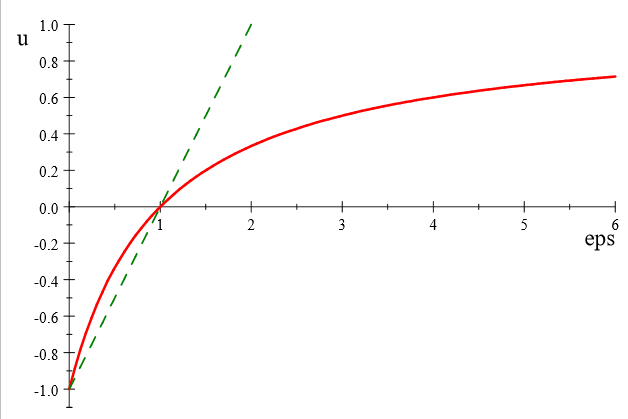
\includegraphics[width=\textwidth]{./Images/Log-Logistic Score.png}
\subsection{Stationarity and Invertibility}
\textbf{Stationarity}\\
Stationarity of the filter follows from $\phi < 1$, Krengel's theorem implies stationarity of $y_t$.\\
\textbf{Invertibility}\\
The Lipschitz coefficient is 
\begin{align*}
    \Lambda_t(\psi) &= \underset{\lambda_{t|t-1}}{sup}\left| \frac{\partial \lambda_{t+1|t}}{\partial \lambda_{t|t-1}} \right| \\
    &= \underset{\lambda_{t|t-1}}{sup}\left| \phi + \frac{\partial \hat{u_t}}{\partial \lambda_{t|t-1}} \right|\\
    &= \underset{\lambda_{t|t-1}}{sup}|\phi-6\kappa b_t (1-b_t)|\\
    &= \left|\phi-\frac{3}{2}\kappa\right| \quad \text{since $x(1-x)$ is maximised at 0.5, with value 0.25}
\end{align*}
The Lyapunov condition is thus satisfied if:
\begin{align*}
    \underset{\nu}{sup} \E \ln \Lambda_t(\psi) &= \E \ln \left|\phi-\frac{3}{2}\kappa\right| < 0\\
    \left|\phi-\frac{3}{2}\kappa\right| &< 1 \quad \text{by Jensen's}\\
    \left|\frac{3}{2}\kappa\right| - |\phi| &< 1 \quad \text{by triangle inequality} \\
    |\kappa| &< \frac{2}{3}(1+|\phi|)
\end{align*}
\end{document}
